\chapter{Introduction}
\textbf{TODO}:
\begin{itemize}
	\item Fix or rewrite Lemma~\ref{lemma:maxmult}.
	\item Consider adding more patterns/generalizations.
	\item Consider fixing Lemma 4.33 (currently commented).
\end{itemize}

A binary matrix (or 0--1 matrix) is a matrix with ones and zeroes as its entries. In the thesis, we only consider binary matrices and so we omit the word binary. We say that a matrix~$M$ contains a matrix~$P$ as an interval minor, if $P$ can be created from $M$ by a sequence of deletion of one-entries and merges of neighboring rows or columns. Otherwise, we say $M$ avoids $P$. To distinguish among matrices and to indicate the relationship, we usually call the matrix~$P$ a \emph{pattern}.

When working with matrices, we always index rows from top to bottom and columns from left to right, starting with one. When we speak about a row~$r$, we mean a row with index $r$. A \emph{line} of a matrix is either a row or a column.

\section{The main results}
While a lot is know about matrices in general, because they can intuitively represent much more complex objects, interval minors are a fairly new topic and so we have a choice of the direction from which we want to approach them.

To get familiar with definitions and pattern avoidance in general, in Chapter~\ref{chap:chars}, we focus on small patterns (having up to four one-entries only) and describe the common structure of matrices avoiding them.

We then turn our focus elsewhere in Chapter~\ref{chap:ops}, and instead of looking for a structure of matrices avoiding a pattern, given a class of matrices (closed under interval minors) we find the smallest set of forbidden patterns that characterizes the class. We introduce the skew sum of two matrices and show that classes of matrices closed under the skew sum can always be described by a finite number of forbidden pattern. Using the operation more, we show that there are also other classes for which this cannot be achieved.

Because it is very useful to study extremal questions like the maximum number of one-entries of a matrix from a given class of matrices, in Chapter~\ref{chap:ints}, we study a variant of such complexity question, where we instead focus on the maximum number~$k$ of appearances of pairs ``01'' and ``10'' on a single line of a matrix from a given class of matrices. We show that even for classes that are described by just one forbidden pattern, $k$ can be unbounded, and we characterize exactly for which pattern this holds. Then we generalize the approach and show what influence an intersection of classes has on the number $k$.

\section{Preliminaries}
\begin{ntn}
For $n\in\mathbb{N}$, let $[n]:=\{1,2,\dots,n\}$ and for $m\in\mathbb{N}$ such that $n\leq m$, let $[n,m]:=\{n,n+1,\dots,m\}$.
\end{ntn}

\begin{ntn}
For a matrix~$M\in\Mat$, $R\subseteq[m]$ and $C\subseteq[n]$, let $M[R,C]$ denote a submatrix of $M$ induced by row indices in $R$ and column indices in $C$. Furthermore, for $r\in[m]$ and $c\in[n]$, let $M[r,c]:=M[\{r\},\{c\}]$.
\end{ntn}

The pattern avoidance for matrices is a generalization of a long studied theory of pattern avoidance for permutations. There are two generally used ways to define this generalization, either we avoid a matrix pattern as a submatrix or as an interval minor. While this thesis works almost exclusively with the latter, to better introduce the whole area, we start by defining the more know of the two approaches.

\begin{defn}
We say a matrix~$M\in\Mat$ \emph{contains} a pattern~$P\in\Pat$ \emph{as a submatrix} and denote it by $\PsmM$ if there are $R\subseteq[m]$ and $C\subseteq[n]$ such that $M'=M[R,C]\in\Pat$ and for every $r\in R$ and $c\in C$, if $P[r,c]=1$ then $M'[r,c]=1$.
\end{defn}

Every matrix~$M\in\Mat$ can be looked at as an adjacency matrix of a bipartite graph $G_M$ with two sets of vertices $V_1=[m]$ and $V_2=[n]$ such that a vertex~$i$ from $V_1$ is adjacent to a vertex $j$ from $V_2$ if and only if $M[i,j]=1$. The order of vertices in each set is fixed and these graphs are usually called ordered bipartite graphs. In this setting, a matrix~$M$ contains a pattern~$P$ if the ordered bipartite graph $G_P$ is a subgraph (not necessarily induced) of the ordered bipartite graph $G_M$.

In graph theory, the next step is to look at graph minors. A minor is created from a graph by a repeated applying of one of three graph operations: deletion of a vertex, deletion of an edge and a contraction of an edge. The same can be represented in terms of matrices:

\begin{defn}
We say a matrix~$M\in\Mat$ \emph{contains} a pattern~$P\in\Pat$ \emph{as an interval minor} and denote it by $\PimM$ if there is a sequence of elementary operations that applied to $M$ creates $P$. The elementary operations are:
\begin{itemize}
	\item a deletion of a line,
	\item a deletion of a one-entry (a change of a one-entry to a zero-entry) and
	\item a merge of two neighboring rows or columns into one that is the elementwise OR of the two original lines. 
\end{itemize}
\end{defn}

For simplicity, we do not consider a deletion of a line to be a separate operation as it can be replaced by a merge of the corresponding line with a neighboring one and a series of changes of one-entries to zero-entries. Moreover, like in the realm of graphs, we can assume all merging operations are done before the deletion of one-entries. This give us an alternative way to look at the problem.

\begin{defn}
Consider matrices $P$ and $M$ and let $P\im M$. A \emph{mapping} of $P$ to $M$ is a function that maps each row of $P$ to an interval of rows of $M$ and each column of $P$ to an interval of columns of $M$ in such a way that if $P[r,c]=1$ and $r$ is mapped to $R$ and $c$ is mapped to $C$, there is a one-entry in $M[R,C]$. An \emph{interval of rows} (columns) is a set of consecutive rows (columns). We say that an entry~$P[r,c]$ is mapped to an entry~$M[r',c']$ in a fixed mapping of $P$ to $M$, in which $r$ is mapped to $R$ and $c$ is mapped to $C$, if $r'\in R$ and $c'\in C$ and if $P[r,c]=1$ then we also require $M[r',c']=1$.
\end{defn}

Each mapping of a pattern~$P$ to a matrix~$M$ corresponds to a \emph{partitioning} of $M$ to intervals of rows and columns that creates a block structure. On the other hand, if we find a partitioning of $M$ to blocks such that for each one-entry $P[r,c]$ there is a one-entry in the block that can be indexed $[r,c]$ then we have a mapping of $P$ to $M$ and so $P\im M$. This means:

\begin{obs}
For all matrices $P$ and $M$, there is a mapping of $P$ to $M\Leftrightarrow\PimM$. \qed
\end{obs}

While pattern avoidance in terms of submatrices and interval minors seem to be very different, they have a quite tight relationship. The next observation immediately follows from their definitions.

\begin{obs}
\label{obs:submin}
For all matrices $P$ and $M$, $\PsmM\Rightarrow\PimM$.
\end{obs}

As said at the beginning of the section, both approaches generalize pattern avoidance for permutations and so it makes sense that they are equal for permutation matrices -- matrices having exactly one one-entry in each line.

\begin{obs}
\label{obs:perm}
For all matrices $P$ and $M$, if $P$ is a permutation matrix then $\PsmM\Leftrightarrow\PimM$.
\end{obs}
\begin{proof}
If we have $\PimM$, then there is a mapping~$m$ of $P$ to $M$. To show $P\leq M$ we need to find $R,C$ such that $M'=M[R,C]$ has the same size as $P$ and for every $P[r,c]=1$ it holds $M'[r,c]=1$. We define $R$ and $C$ as follows. For every row~$r$, let $R'$ be the interval to which $r$ is mapped in the mapping~$m$. There is exactly one column~$c$ such that $P[r,c]=1$ and $c$ is mapped to some $C'$. Because $m$ is a mapping, there is a one-entry $M[r',c']$ such that $r'\in R'$ and $c'\in C'$ and we add $r'$ to $R$ and we add $c'$ to $C$.

The other implication follows from Observation~\ref{obs:submin}.
\end{proof}

\begin{defn}
A \emph{class} of matrices~$\class{M}$ is a set of matrices that is closed under interval minors. It means that for every $M\in\class{M}$ and every $M'\im M$ it holds $M'\in\class{M}$.
\end{defn}

To avoid degenerate cases, we only consider classes of matrices containing at least one matrix of size $2\times1$, at least one matrix of size $1\times2$ and at least one matrix that is non-empty.

\begin{defn}
Let $\class{P}$ be a set of patterns. We denote by $\Avm{\class{P}}$ the set of all matrices that avoid each $P\in\class{P}$ as an interval minor.
\end{defn}

\begin{obs}
\label{obs:im}
For all patterns $P$ and $P'$: $P\im P'\Leftrightarrow\Avm{P}\subseteq\Avm{P'}$.
\end{obs}
\begin{proof}
Because $P\im P'$, every matrix that avoids $P$ also avoids $P'$. On the other hand, if $P\nim P'$ then $P'\in\Avm{P}$. As $P'\not\in\Avm{P'}$, we have $\Avm{P}\not\subseteq\Avm{P'}$.
\end{proof}

The following observation goes almost without saying and we use it throughout the whole thesis to break symmetries.

\begin{obs}
Let $P$ and $M$ be matrices, $\PimM\Leftrightarrow P^T\im M^T$.
\end{obs}

\section{Pattern avoidance}
Pattern avoidance is a general topic in combinatorics. A lot of attention is directed towards permutations, see books \cite{bona, kitaev} for references. It is a natural generalization to regard permutations as permutation matrices and consider matrix avoidance. This is mainly studied in terms of submatrices, so we discuss some interesting results in this section.

Interval minors are, on the other hand, a fairly new topic first defined by Jacob Fox in \cite{fox} as a tool to prove results about permutations in the study of Stanley--Wilf limits. Since then, a little has been discovered about the theory of interval minors. Nevertheless, we mention some results at the end of this section.

Let us go back to submatrices for now. The question that is particularly interesting is to determine the maximum number of one-entries that a matrix avoiding a given pattern can have. This property describes complexity of a pattern and can be used for example to prove algorithmic complexity, see \cite{efrat}.

\begin{defn}
Let $M$ be a matrix. The weight of $M$, denoted by $|M|$, is the number of one-entries in $M$.
\end{defn}

\begin{defn}
For a pattern~$P$ and integers $m,n$, we define the \emph{weight extremal function}~$Ex(P,m,n):=\max\{|M|;\ M\in\Mat\wedge\PnsmM\}$.
\end{defn}

Going back to the representation of the problem in terms of ordered bipartite graphs, the question to determine $Ex(P,m,n)$ is a variant of a classical Tur{\'a}n extremal graph question and was studied by many authors, see for example \cite{tardos, furedi} or, for a wider range of variants \cite{brass, claesson, klazar, pach}. Some applications associated with the weight extremal function are discussed in \cite{fulek}. There are other extremal functions that have been studied, see for instance \cite{kyncl}, but we do not consider them in this thesis.

In the same spirit, we also define the weight extremal function for matrices avoiding patterns as interval minors.

\begin{defn}
For a pattern~$P$ and integers $m,n$, we define $Ex_{\preceq}(P,m,n):=\max\{|M|;\ M\in\Mat\wedge\PnimM\}$.
\end{defn}

Thanks to Observation~\ref{obs:submin} we have the following relationship between the extremal functions.

\begin{obs}
\label{obs:exm<ex}
For all patterns~$P$ and integers $m,n$:

$Ex_{\preceq}(P,m,n)\leq Ex(P,m,n)$. \qed
\end{obs}

From Observation~\ref{obs:im} it follows:

\begin{obs}
For all patterns~$P$ and $P'$ and integers $m,n$: $P\im P'\Rightarrow Ex_{\preceq}(P,m,n)\leq Ex_{\preceq}(P',m,n)$.
\end{obs}

It was showed in \cite{Marcus} that for every permutation matrix~$P$ and every $n$ it holds $Ex(P,n,n)\leq c_Pn$. While $Ex(P,n,n)$ can become even quadratic with $n$, because of the previous observation and the fact that every pattern~$P\in\Pat$ is an interval minor of some permutation pattern~$P'\in\bin^{(kl)\times(kl)}$ we have the following:

\begin{prop}
For every pattern~$P$ and integer~$n$: $Ex_{\preceq}(P,n,n)\leq c_Pn$ for some constant $c_P$ independent of $n$. \qed
\end{prop}

The following observation for $Ex(P,m,n)$ was made by several authors; see for example \cite{cibulka09, fulek}.

\begin{lemma}
If $P\in\{0,1\}^{k\times l}$ has at least one one-entry, then

$Ex(P,m,n)\geq\Big\{\begin{array}{ll}
m\cdot n & k>m\text{ or } l>m \\
(k-1)n+(l-1)m-(k-1)(l-1) & \text{otherwise.}
\end{array}$

Moreover, the same holds for $Ex_{\preceq}(P,m,n).$
\end{lemma}
\begin{proof}
If $k>m\vee l>m$, we have $P\nim\{1\}^{m,n}$. Otherwise, let $P[r,c]=1$ and consider Figure~\ref{fig:minimalist}. Consider a matrix~$M$ such that the first $r-1$ rows, the last $k-r$ rows, the first $c-1$ column and the last $l-c$ column contain no zero-entry and the rest is empty. Then $P\not\leq M$ and even $P\nim M$. We can also see that $|M|=mn-(m-k+1)(n-l+1)=(l-1)m+(k-1)n-(k-1)(l-1)$.
\end{proof}
\begin{figure}[!ht]
\centering
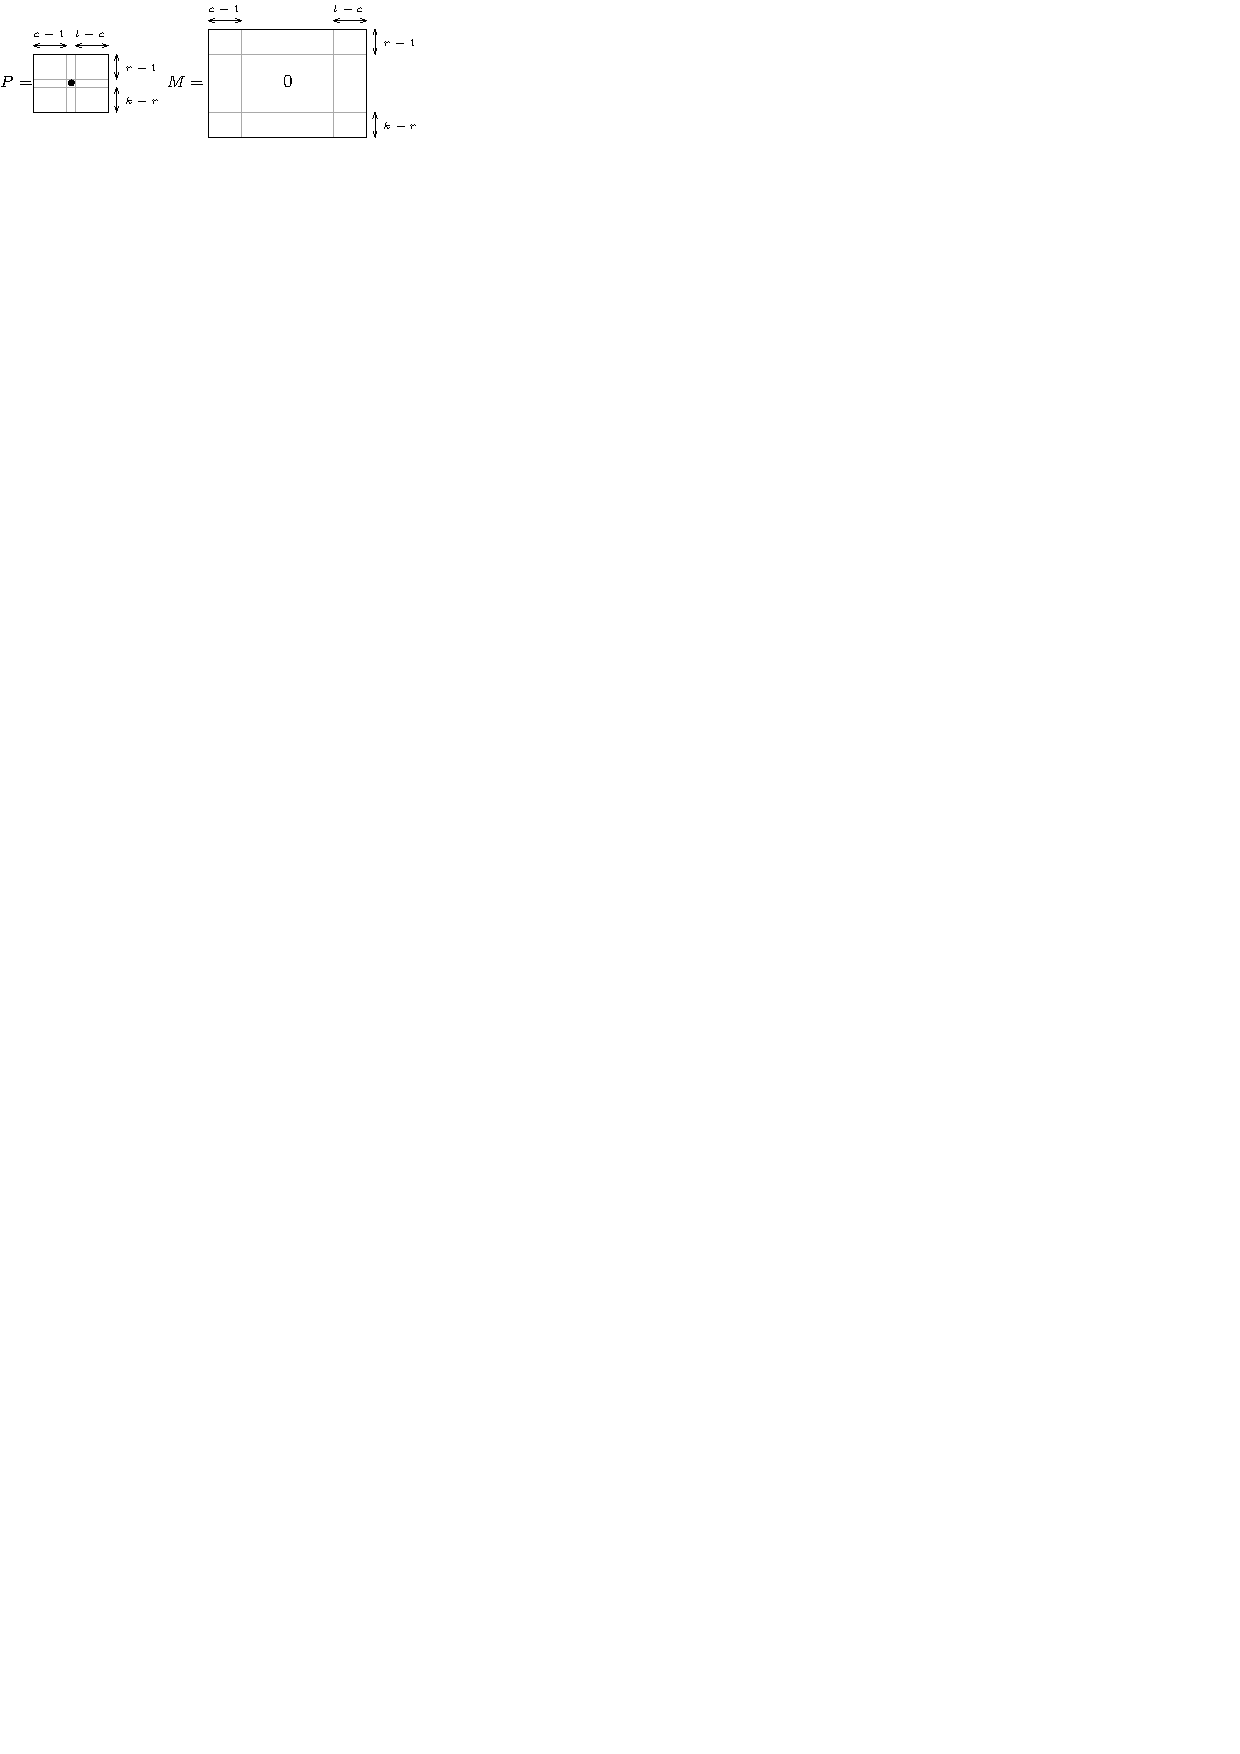
\includegraphics[width=120mm]{img/minimalist.pdf}
\caption{An example of a matrix~$M$ avoiding a pattern~$P$ as an interval minor.}
\label{fig:minimalist}
\end{figure}

The following definition is due to \cite{cibulka}.

\begin{defn}
A pattern~$P\in\{0,1\}^{k\times l}$ is \emph{(strongly) minimalist} if
$$Ex(P,m,n)=\Big\{\begin{array}{ll}
m\cdot n & k>m\text{ or } l>m \\
(k-1)n+(l-1)m-(k-1)(l-1) & \text{otherwise.}
\end{array}$$
\end{defn}

We use the adjective ``strongly'' to further distinguish minimalist pattern from weakly minimalist patterns defined next.

\begin{defn}
A pattern~$P\in\{0,1\}^{k\times l}$ is \emph{weakly minimalist} if
$$Ex_{\preceq}(P,m,n)=\Big\{\begin{array}{ll}
m\cdot n & k>m\text{ or } l>m \\
(k-1)n+(l-1)m-(k-1)(l-1) & \text{otherwise.}
\end{array}$$
\end{defn}

From Observation~\ref{obs:exm<ex}, we immediately have:

\begin{obs}
\label{obs:strongweak}
If a pattern~$P$ is strongly minimalist then $P$ is weakly minimalist.
\end{obs}

The following result is a simplification of a lemma from \cite{cibulka}.

\begin{fct}
\label{fct:minimalist}
\begin{enumerate}
	\item The pattern~$\smm{\bullet}$ is strongly minimalist.
	\item If a pattern~$P\in\Pat$ is strongly minimalist and there is a one-entry in the last row of $P$ in the $c$-th column, then $P'\in\{0,1\}^{k+1\times l}$ created from $P$ by appending as the last row a new row having a one-entry only in the $c$-th column is strongly minimalist.
	\item If a pattern~$P$ having at least two one-entries is strongly minimalist, then after changing a one-entry to a zero-entry it is still strongly minimalist.
\end{enumerate}
\end{fct}

The following two facts come from \cite{bigraphs}. In the article, a slightly different definition of an interval minor is used, so we show here the proofs in our setting.

\begin{fct}[\cite{bigraphs}]
\label{fct:2weak}
Let $P=\{1\}^{2\times l}$ be a pattern, then $P$ is weakly minimalist.
\end{fct}
\begin{proof}
Let $M\in\Mat$ be a matrix avoiding $P=\{1\}^{2\times l}$ as an interval minor and let $A_i$ be the set of column indices $j$ such that both $M[[i],\{j\}]$ and $M[[i+1,m],\{j\}]$ are non-empty. Clearly, $|A_i|\leq l-1$; otherwise, $P\preceq M$. Let $b_j$ denote the number of one-entries in the $j$-th column. Each column~$j$ of $M$ appears in at least $b_j-1$ of sets $A_i$, $1\leq i\leq m-1$. It follows that

$|M|=\sum\limits_{j=1}^nb_j=\sum\limits_{j=1}^n(b_j-1)+n\leq\sum\limits_{i=1}^{m-1}|A_i|+n\leq(l-1)(m-1)+n$.
\end{proof}

This result shows an example of a weakly minimalist matrix that is not strongly minimalist. Consider a matrix~$\smm{\bullet&\bullet\\\bullet&\bullet}$. It is, thanks to Fact~\ref{fct:2weak} weakly minimalist, but it is known due to \cite{p33} that it is not strongly minimalist.

\begin{fct}[\cite{bigraphs}]
\label{fct:3weak}
Let $P=\{1\}^{3\times l}$ be a pattern, then $P$ is weakly minimalist.
\end{fct}
\begin{proof}
Let $M\in\Mat$ be a matrix avoiding $P=\{1\}^{3\times l}$ as an interval minor and let $A_i$ be a set of column indices $j$ such that both $M[[i-1],\{j\}]$ and $M[[i+1,m],\{j\}]$ are non-empty and $M[i,j]=1$. Clearly $|A_i|\leq l-1$, otherwise $P\preceq M$. Let $b_j$ denote the number of one-entries in the $j$-th column. Each column~$j$ of $M$ (for which $b_j\geq2$) appears in exactly $b_j-2$ of sets $A_i$, $2\leq i\leq m-1$. It follows that

$|M|=\sum\limits_{j=1}^nb_j=\sum\limits_{j=1}^n(b_j-2)+2n\leq\sum\limits_{i=2}^{m-1}|A_i|+2n\leq(l-1)(m-2)+2n$.
\end{proof}

We now show that the third part of Fact~\ref{fct:minimalist} is also safe for weakly minimalist patterns.

\begin{lemma}
Let $P\in\Pat$ be a weakly minimalist pattern having at least two one-entries. Then a pattern~$P'$ created from $P$ be deletion of a one-entry is also weakly minimalist.
\end{lemma}
\begin{proof}
For contradiction, consider a matrix~$M\in\Mat$ avoiding $P'$ as an interval minor such that $|M|>(k-1)n+(l-1)m-(k-1)(l-1)$. The matrix~$M$ also avoids $P$; as otherwise, we have $P'\im P\im M$. That is a contradiction with $P$ being weakly minimalist. 
\end{proof}

As a result, we have the following corollary:

\begin{cor}
Every non-empty pattern~$P$ that has at most three rows (or columns) is weakly minimalist.
\end{cor}

In \cite{cibulka09}, the author shows that for every $k\geq1$ there is a $2k\times2k$ permutation pattern for which $Ex[P,n]\geq k^2n$. Because of Observation~\ref{obs:perm}, the same construction shows that for $k\geq2$ the patterns are not weakly minimalist. It means that the previous results cannot be easily extended. On the other hand, in \cite{multipartite} the authors show some form of generalization and also other bounds regarding interval minors and their weight extremal function.